\documentclass[twoside,12pt]{article}\usepackage[includemp=true,marginparsep=.5cm,marginparwidth=3cm,left=1.7cm,right=.7cm,top=2cm,bottom=1.5cm]{geometry}\newtheorem{Definition}{定义}[section]

%\documentclass[mathserif,blue]{beamer}%handout
\def\aim{\begin{itemize*}
    \item 会使用平面向量的数量积的定义及其几何意义
    \item 能说出平面向量数量积的重要性质及运算律
    \item 了解用平面向量的数量积可以处理有关长度、角度和垂直的问题
  \end{itemize*}}



\usepackage[includemp=true,marginparsep=.5cm,marginparwidth=3cm,left=.7cm,right=1.7cm,top=2cm,bottom=1.5cm]{geometry}
\usepackage{amsmath,amssymb}
\usepackage{stmaryrd}
\usepackage{verbatim}
\usepackage{mdwlist}%提供紧凑的列表
\usepackage{graphicx}
\usepackage{tikz}
\usepackage{ifthen}
\usepackage[colorlinks=true,linkcolor=blue,citecolor=blue]{hyperref}
\usepackage{xfrac}%提供斜分数命令,\sfrac{1}{3}
\usepackage{ctex}
%\usepackage{titlesec}%标题格式
\usepackage{fancyhdr}%页眉页脚
\usepackage{listings}%插入代码
\usepackage{framed}
\usepackage{lipsum}
\usepackage{subfig}%子图
\usepackage{tabularx,booktabs}%插入表格
\usepackage{indentfirst} %首行缩进
\usepackage{array} 
\usepackage{longtable}%长表格
\usepackage{multirow}%使用多栏宏包
\usepackage{wrapfig}%文字环绕
\usepackage{extarrows}
\usepackage{ulem,bm}
\usepackage{cite}%参考文献
\usepackage[super,square,comma,sort&compress]{natbib} 
\usepackage{setspace}%设定行距

\setCJKfamilyfont{huawen}{STXihei}
\setCJKfamilyfont{hwzhs}{STZhongsong}
\newcommand\xihei{\CJKfamily{huawen}} %华文细黑
\newcommand\zhongsong{\CJKfamily{hwzhs}}%华文中宋
\usetikzlibrary{arrows,arrows.spaced,arrows.meta,calc,intersections,through,backgrounds,math,angles,shapes}

\newtheorem{theorem}{定理}
\newtheorem{definition}{\hei 定义}
\newtheorem{property}{问题}
\newtheorem{proposition}{猜测}
\newtheorem{lemma}{引理}
\newtheorem{corollary}{推论}

\newcommand\Dd{\displaystyle}\newcommand{\Tt}{\textstyle}\newcommand{\Ss}{\scriptstyle}\newcommand{\Sss}{\scriptscriptstyle}%
\setlength\mathsurround{0.5ex}%数学模式与文本模式混排时留出的间距
\newcommand\an[1][a]{\ensuremath{\{#1_n\}}}%sequence
\newcommand\ud{\mathrm{d}}
\newcommand{\ue}{\mathrm{e}}%正体字母
\newcommand\triabc{\ensuremath{\triangle ABC}}%三角形ABC
\newcommand\cnm[2][n]{\ensuremath{\textrm{C}^{#2}_{#1}}}%组合数
%数学题目编辑
\newcommand\lines[1][1.2]{\,\underline{\mbox{\hspace{#1cm}}}\,}% 填空题的横线
\newcommand\brackets[1][2]{\nolinebreak\hfill\mbox{~(\hspace{#1em})}\\}% 选择题的括号
%扩展命令
\newcommand\qqquad{\qquad\quad}
\def\aside#1{\marginpar{\footnotesize #1}}
%自动编号之最简
\newcommand\numa{\refstepcounter{numi}\thenumi}\newcounter{numi}
\newcommand\numb{\refstepcounter{numii}\thenumii}\newcounter{numii}
\newcommand\numc{\refstepcounter{numiii}\thenumiii}\newcounter{numiii}
\newcommand\numaa{\refstepcounter{numai}\thenumai}\newcounter{numai}[numi]

\newcommand{\question}[1][]{\par\vspace{1ex}\noindent\refstepcounter{numberi}\textbf{\thenumberi.}\ensuremath{#1}}\newcounter{numberi}[subsection]% 每道小题自动编号
\newcommand\quson{\\ \hspace*{1em}\refstepcounter{numberii}\thenumberii)~}\newcounter{numberii}[numberi]% 每道小题自动编号
\newcommand\choice[5][4]{\vspace*{-1em}\begin{tasks}(#1)\task$#2$\task$#3$\task$#4$\task$#5$\end{tasks}\vspace*{-1.2em}}%选择题排版之数学模式
\newcommand\choicex[5][4]{\vspace*{-1em}\begin{tasks}(#1)\task#2\task#3\task#4\task#5\end{tasks}\vspace*{-1.2em}}%选择题排版之数学模式
\newcommand\tbs[1][]{\texttt{\char92#1}}
\newcommand\bpics[1]{\par\vspace{1ex}\noindent\begin{minipage}{\textwidth}\begin{minipage}{#1\textwidth}}
\newcommand\mpics[1]{\end{minipage}\begin{minipage}{#1\textwidth}\linespread{1}}
\newcommand\epics{\end{minipage}\end{minipage}\par\vspace{2ex}}

\newcommand\set[1]{\lbrace\ensuremath{#1}\rbrace}
\newcommand\setx[1]{\{#1\}}

\newcommand\mybf[1]{{\bm#1}}
\def\bfR{\mybf R}
\def\bfN{\mybf N}
\def\bfZ{\mybf Z}
\def\bfQ{\mybf Q}
\def\bfC{\mybf C}
\def\bfZp{\mybf Z^+}

\newcommand\myvec[1]{\bm#1}
\def\veca{\myvec a}
\def\vecb{\myvec b}
\def\vecc{\myvec c}
\def\vecd{\myvec d}
\def\vece{\myvec e}
\def\vecf{\myvec f}
\def\vecs{\myvec e}
\def\vecp{\myvec p}
\def\vecq{\myvec q}
\def\veci{\myvec i}
\def\vecj{\myvec j}
\def\vecei{\myvec{e_1}}
\def\veceii{\myvec{e_2}}
\def\veczero{\myvec 0}
\newcommand\lvec[1]{\overrightarrow{#1}}
%background rectangle/.style={draw=blue!50,fill=blue!20,rounded corners=1ex},show background rectangle

%\begin{columns}\begin{column}{\.5\textwidth} \end{column}\begin{column}{.5\textwidth} \end{column}\end{columns}

%受命于tikz
\def\mystyle{\tikzset{myvec/.style={-stealth}}}
%兼容于beamer
\def\pause{}

%%%listings设置    \begin{lstlisting} !!code!! \end{lstlisting}
\lstset{
        numbers=none, %设置行号位置
       numberstyle=\wuhao, %设置行号大小
        keywordstyle=\color{blue}, %设置关键字颜色
        commentstyle=\color[cmyk]{1,0,1,0}, %设置注释颜色
        %frame=shadowbox, %设置边框格式
        escapeinside=``, %逃逸字符(1左面的键),用于显示中文
        breaklines, %自动折行
        extendedchars=false, %解决代码跨页时,章节标题,页眉等汉字不显示的问题
        xleftmargin=0em,xrightmargin=0em, aboveskip=0.5em,%设置边距
        framextopmargin=0pt,framexbottommargin=2pt,abovecaptionskip=-3pt,
        belowcaptionskip=0pt,  
        %tabsize=1, %设置tab空格数
        showspaces=false %不显示空格
        commentstyle=\color{red!50!green!50!blue!50},%浅灰色的注释  
        keywordstyle=\color{blue!90}\bfseries, %代码关键字的颜色为蓝色,粗体  
        rulesepcolor=\color{red!20!green!20!blue!20},%代码块边框为淡青色  
        numberstyle={\color[RGB]{255,1,1}\scriptsize} ,%设置行号的大小,大小有tiny,scriptsize,footnotesize,small,normalsize,large等  
        numbersep=8pt,  %设置行号与代码的距离,默认是5pt  
  basicstyle=\footnotesize, % 这句设置代码的大小  
        frame=shadowbox, %把代码用带有阴影的框圈起来  
        backgroundcolor=\color[RGB]{245,245,244},   %代码背景色         
       }
%\usepackage[includemp=true,marginparsep=.5cm,marginparwidth=3cm,left=2.5cm,right=2cm]{geometry}%带有旁注marginpar
%\usepackage[paperheight=6in,paperwidth=4.5in,margin=1cm]{geometry}%kindel专用

\begin{document}

%\setcounter{page}{2}\pagestyle{empty}
\def\myp#1{\par\vspace*{1ex}\noindent{\heiti#1}\par}\def\myskip{\par\vspace*{.7in}}
\centerline{\heiti\Large 平面向量的数量积导学案 第一课时}

\section{学习目标}
 \begin{itemize*}
    \item 会使用平面向量的数量积的定义及其几何意义
    \item 能说出平面向量数量积的重要性质及运算律
    \item 了解用平面向量的数量积可以处理有关长度、角度和垂直的问题
  \end{itemize*}

\section{数量积的物理背景}
在初中物理上,功等于\textsl{力与位移的乘积}. 这个定义仅适用于力与位移在同一个方向上时. 在高中,功被定义为\textsl{力和物体在力的方向上的位移的乘积},计算公式为 $W=Fs\cos\theta$.\aside{向上的分力不做功,就像水蒸气一样蒸发了}\par 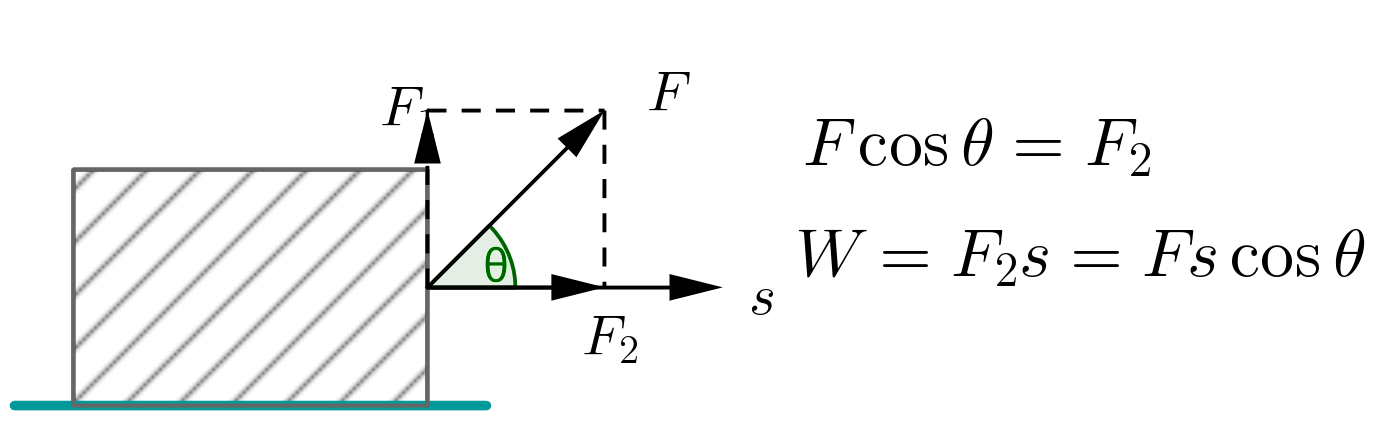
\includegraphics[width=3.5in]{d241-01.png}
\aside{ 这是不是意味着两个向量的乘积是一个数量?\\答:两个向量的数量积(也叫内积)是一个数量. }
力是一个向量,位移也是一个向量,而力在物体位移的方向上所做和功是一个标量,这可以说是我们定义两个向量的数量积的出发点.

 
\section{数量积的定义}
\aside{ 为什么叫数量积呢?叫点乘积岂不更好!因为两个向量运算的结果是一个数,所以叫数量积.} 
\begin{definition}向量$\veca,\vecb$的数量积$$\veca\cdot\vecb=|\veca||\vecb|\cos\theta$$
其中$\theta$是$\veca$与$\vecb$的夹角. 我们规定,零向量与任一向量的数量积为$0$
\end{definition}\aside{ 为什么要加一条规定呢?只是因为零向量与任意向量的夹角任意,没有办法计算$\cos\theta$.}

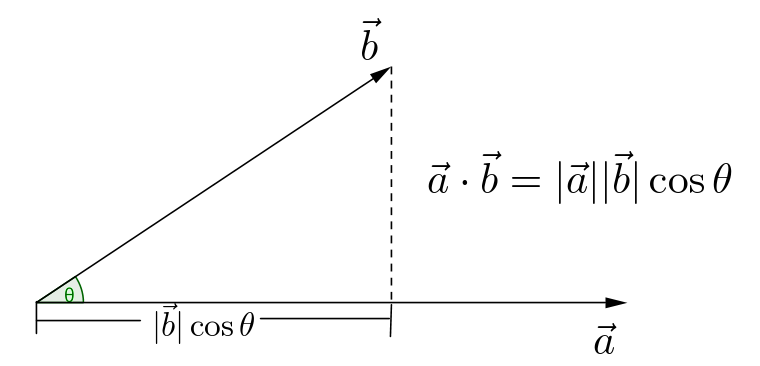
\includegraphics[width=3.3in]{d241-02.png}


\textbf{注意}:中间的“$\cdot$”不可以省略,也不可以写成“$\times$”.


例1.已知$|\veca|=5$, $|\vecb|=4$,$\veca$与$\vecb$的夹角$\theta=120^\circ$,求$\veca\cdot\vecb$.\vspace{2ex}

 
练习1.已知$|\vecp|=8$, $|\vecq|=6$,  向量$\vecp$ 和 $\vecq$的夹角是$60^\circ$, 求 $\vecp\cdot\vecq$.

\myskip
练习2.设$|\veca|=12$,$|\vecb|=9$, $\veca\cdot\vecb=−54$,求向量$\veca$和$\vecb$的夹角$\theta$.
\myskip 

\section{数量积的性质}
\myp{思考}
1.向量的数量积什么时候为正,什么时候为负?
\aside{ 老师,你问的要是非零向量就好了. }
\myskip
   
2.$|\veca\cdot\vecb|$与$|\veca||\vecb|$之间有不等关系吗?
\aside{ 反正不是相等关系.}
\myskip

\myp{数量积的性质}\vspace{1ex}
\hrule\vspace{1ex}
  设$\veca,\vecb$都是非零向量, 
$\theta$是$\veca$与$\vecb$的夹角,则
  \begin{itemize*}
    \item $\veca\perp\vecb\iff\veca\cdot\vecb=0$\quad(判断两向量垂直的依据)
    \item 当$\veca$与$\vecb$同向时,$\veca\cdot\vecb=|\veca||\vecb|$,
     当$\veca$与$\vecb$反向时, $\veca\cdot\vecb=−|\veca||\vecb|$.特别地,$\veca\cdot\veca=|\veca|^2$或$|\veca|=\sqrt{\veca\cdot\veca}$\quad(用于计算向量的模)
    \item $|\veca\cdot\vecb|\le|\veca|\cdot|\vecb|$\quad 一个常用不等式
  \end{itemize*}
\hrule\vspace{1ex}

例2.判断正误\begin{itemize*}\def\mybra{\quad(\quad)}
  \item 若$\veca=\veczero$,则对任一向量$\vecb$,有$\veca\cdot\vecb=0$.\mybra
  \item 若$\veca\ne\veczero,\vecb\ne\veczero$,则有$\veca\cdot\vecb\ne0$.\mybra
  \item 若$\veca\ne\veczero, \veca\cdot\vecb=0$,则 $\vecb=\veczero$.\mybra
  \item 若$\veca\cdot\vecb=0$,则$\veca,\vecb$中至少有一 个 为 $\veczero$.\mybra
  \item 若$\vecb\ne\veczero$,且$\veca\cdot\vecb=\vecb\cdot\vecc$,则 $\veca=\vecc$.\mybra
  \item 对任意向量$\veca$ ,有$\veca^2=|\veca|^2$.\mybra \aside{ 符号$\veca^2$尚未定义,这里假定聪明的你明白是什么意思}
\end{itemize*}
\vfill
\section{数量积的几何意义}
平面向量数量积 $\veca\cdot\vecb$的几何意义

定义$\veca\cdot\vecb=|\veca||\vecb|\cos\theta$中,$|\veca|\cos\theta$叫做向量$\veca$在$\vecb$上的\textbf{投影},$|\vecb|\cos\theta$叫做向量$\vecb$在$\veca$上的\textbf{投影}. 

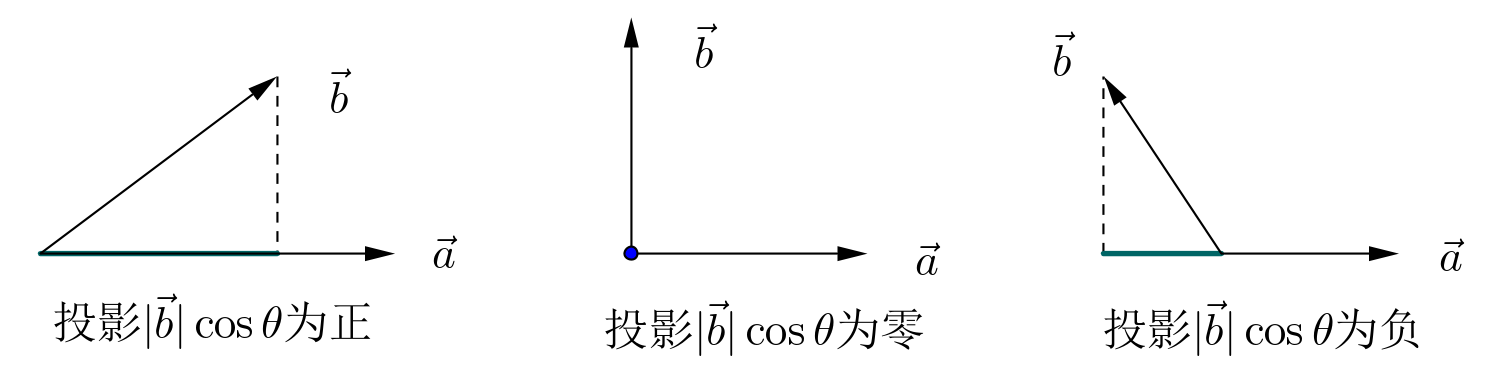
\includegraphics[width=5.5in]{d241-03.png}

向量 $\veca$ 与$\vecb$ 的数量积等于$\veca$ 的长度 $|\veca|$ 与$\vecb$ 在$\veca$ 的方向上的投影$|\vecb|\cos\theta$的积.


\section{运算律}
\myp{数量积运算律}\hrule\vspace{1ex}
  \begin{enumerate*}
    \item $\veca\cdot\vecb=\veca\cdot\vecb$\quad 交换律
    \item $(\lambda\veca)\cdot\vecb=\lambda(\veca\cdot\vecb)=\veca\cdot(\lambda\vecb)$ \quad 与数的结合律
    \item $(\veca+\vecb)\cdot\vecc=\veca\cdot\vecc+\vecb\cdot\vecc$\quad 分配律
\aside{ 学了数量积的坐标表示再来证明分配律,会容易得多.}
  \end{enumerate*}
\hrule\vspace{1ex}
    \par 思考:\aside{ 老师,放这里是分明地暗示不成立呀!}$(\veca\cdot\vecb)\cdot\vecc=\veca\cdot(\vecb\cdot\vecc)$ 成立吗?为什么?
\myskip


 
例3.求证:(1)$(\veca +\vecb)^2=\veca^2+2\veca\cdot\vecb+\vecb^2$\par     
(2)$(\veca+\vecb)\cdot(\veca-\vecb)=\veca^2-\vecb^2$
\myskip
  
例4.已知$|\veca|=6,|\vecb|=4$,$\veca$与$\vecb$的夹角为$60^\circ$,求$(\veca+2\vecb)\cdot(\veca-3\vecb)$.
\newpage

\section{数量积的几点应用}
\subsection{判断两个向量是否垂直}
例5.已知$|\veca|=3, |\vecb|=4$(且$\veca$与$\vecb$不共线),且仅当$k$为何值时,向量$\veca+k\vecb$与$\veca-k\vecb$互相垂直?\aside{边注这么多空白,不拿来演草岂不可惜.}
\myskip
变式训练1:若向量$\veca,\vecb,\vecc$满足$\veca\sslash\vecb$且$\veca\perp\vecc$,
则$\vecc\cdot(\veca+2\vecb)=$\lines.
\subsection{求向量之间的夹角}
例6.设$\veca,\vecb$是两个不共线的非零向量,且$|\veca|=|\vecb|=|\veca-\vecb|$,求向量$\veca$与$\veca+\vecb$的夹角
\myskip
变式训练2:已知$|\veca|=|\vecb|=2$, $(\veca+2\vecb)\cdot(\veca-\vecb)=-2$, 则$\veca$与$\vecb$的夹角为\lines.
\myskip
%\subsection{用基向量计算}
%例6.设$x,y$轴正方向上的单位向量分别为$\veci$和$\vecj$,若$\veca+\vecb=2\veci-8\vecj$,$\veca-\vecb=-8\veci+16\vecj$,  求$\veca\cdot\vecb$.
%\myskip
%变式训练.设$\vecei$和$\veceii$是夹角为$45^\circ$的两个单位向量,且$\veca=\vecei+2\veceii$,$\vecb=2\veci+\veceii$试求$|\veca+\vecb|$的值.
%\myskip

\section{小结}
\begin{itemize*}
  \item 向量的数量积的物理模型是力的做功.
  \item $\veca\cdot\vecb$的结果是个数量.
  \item 数量积满足交换律,分配律,与数
的结合律,但是不满足结合律
  \item 利用数量积可以求两向量的夹角,特别是可以判定垂直.
\end{itemize*}
变式训练答案:1.\underline{~0~} 2.\underline{~$\pi/3$~}

\end{document}
\songti\mytitle{向量的数量积及运算律}

%\begin{frame}{思考}加法\quad $\veca+\vecb$ \quad 力(位移等)的合成\par
%减法 \quad $\veca-\vecb=\veca+(-\vecb)$ \quad 加法的逆运算\par
% 数乘 \quad $2\veca=\veca+\veca$ \quad 推广到$\lambda\veca$\par
% 两个向量之间在没有乘法运算呢?
%  $$\veca\cdot\vecb=?$$\end{frame}

 
%物理上,力是一个向量,位移也是一个向量,而力在物体位移的方向上所做和功是一个标量,这就是两个向量的积的例子
\begin{frame}{数量积的物理背景}
  力和物体在力的方向上的位移的乘积叫做功,计算公式为 $W=Fs\cos\theta$.\par 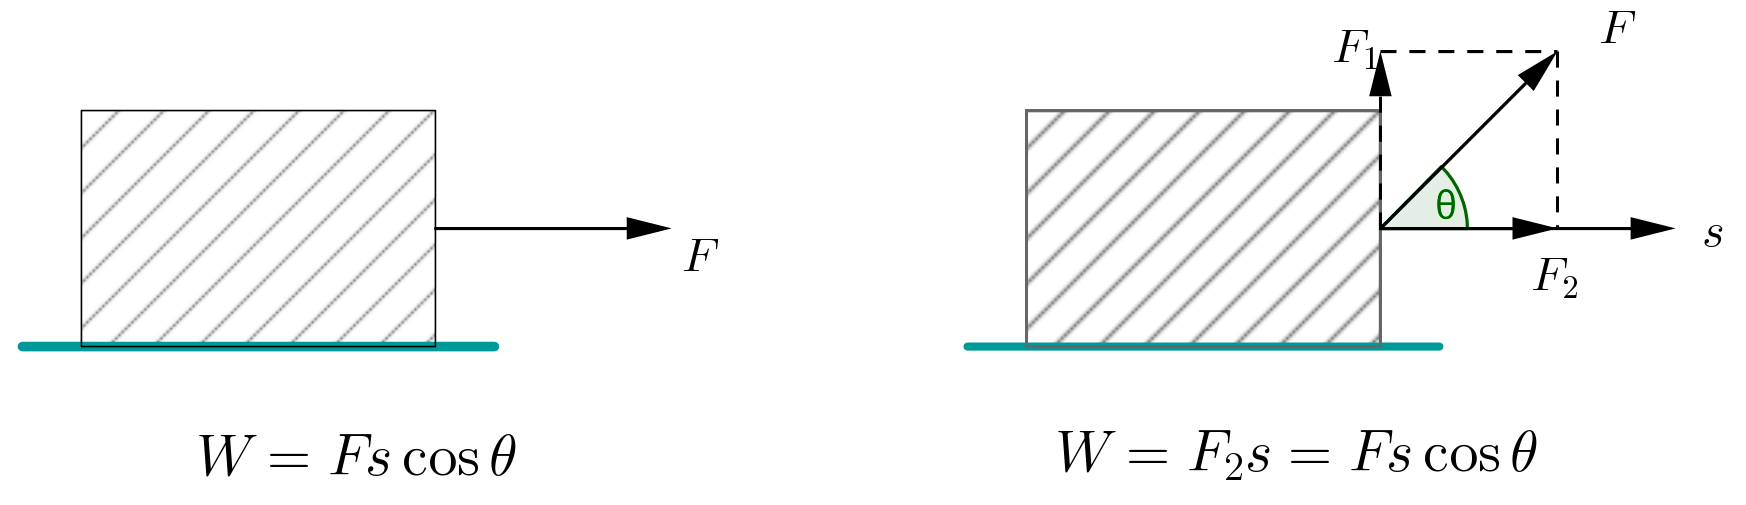
\includegraphics[width=3in]{d241-04.png}
\end{frame}

\begin{frame}
 \begin{block}{学习目标}
  \begin{itemize}
    \item 会使用平面向量的数量积的定义及其几何意义
    \item 能说出平面向量数量积的重要性质及运算律
    \item 了解用平面向量的数量积可以处理有关长度、角度和垂直的问题
  \end{itemize}\end{block}
\end{frame}


\begin{frame}
  \begin{block}{定义:向量的数量积}\bpics{.5}
定义$$\veca\cdot\vecb=|\veca||\vecb|\cos\theta$$
其中$\theta$是$\veca$与$\vecb$的夹角. \\
\emph{我们规定,零向量与任一向量的数量积为$0$.}
\mpics{.5}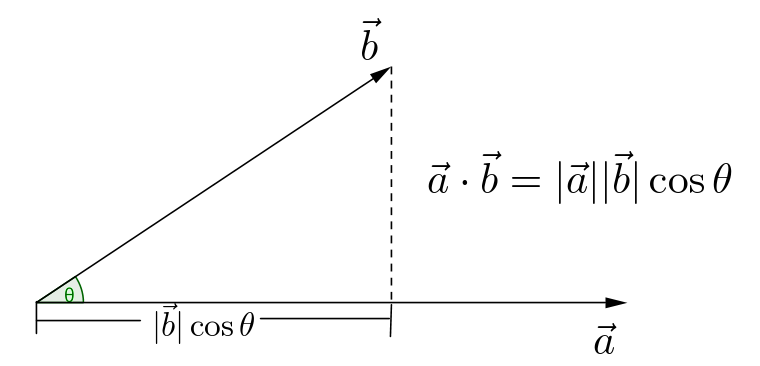
\includegraphics[width=2in]{d241-02.png}\epics
  \end{block}
\end{frame}


\begin{frame}
\begin{exampleblock}{例1}
已知$|\veca|=5$, $|\vecb|=4$,$\veca$与$\vecb$的夹角$\theta=120^\circ$,求$\veca\cdot\vecb$.
\end{exampleblock}\pause
解:$\veca\cdot\vecb=|\veca||\vecb|\cos\theta$\\\pause
\hspace*{4em}$=5\times4\times\cos120^\circ$\\\pause
\hspace*{4em}$=-10$\end{frame}


\begin{frame}
练习1.已知$|\vecp|=8$, $|\vecq|=6$,  向量$\vecp$ 和 $\vecq$的夹角是$60^\circ$, 求 $\vecp\cdot\vecq$.\par\vspace*{3em}
练习2.设$|\veca|=12$,$|\vecb|=9$, $\veca\cdot\vecb=−54$,求向量$\veca$和$\vecb$的夹角$\theta$.\par\pause
答案:1.\underline{~24~}\quad2.\underline{~$2\pi/3$~}
\end{frame}

\begin{frame}{思考}
1.向量的数量积什么时候为正,什么时候为负?\par
\vspace*{6em}
 
2.$|\veca\cdot\vecb|$与$|\veca||\vecb|$之间有不等关系吗?\par\pause
\vspace*{-7em}
答:当$0\le\theta<\pi/2$时,$\veca\cdot\vecb>0$;\par\pause
当$\pi/2<\theta\le\pi$时,$\veca\cdot\vecb<0$;\par\pause
当$\veca\perp\vecb$时,$\veca\cdot\vecb=0$. \par\pause
\vspace*{2.5em}
答:$|\veca\cdot\vecb|\le|\veca||\vecb|$, \pause
等号当且仅当$\veca=\pm\vecb$时取到,$|\veca\cdot\veca|=|\veca|^2$, 此公式可以计算向量的模$|\veca|=\sqrt{\veca^2}$.
\end{frame}


\begin{frame}{数量积的性质}
\begin{block}{}设$\veca,\vecb$都是非零向量,$\theta$是$\veca$与$\vecb$的夹角,则
  \begin{itemize}[<+->]
    \item $\veca\perp\vecb\iff\veca\cdot\vecb=0$(判断两向量垂直的依据)
    \item 当$\veca$与$\vecb$同向时,$\veca\cdot\vecb=|\veca||\vecb|$,
     当$\veca$与$\vecb$反向时, $\veca\cdot\vecb=−|\veca||\vecb|$.特别地,$\veca\cdot\veca=|\veca|^2$或$|\veca|=\sqrt{\veca\cdot\veca}$(用于计算向量的模)
    \item $|\veca\cdot\vecb|\le|\veca|\cdot|\vecb|$
  \end{itemize}\end{block}
\end{frame}


\begin{frame}
 \begin{exampleblock}{例2.判断正误}\begin{itemize}
  \item 若$\veca=\veczero$,则对任一向量$\vecb$,有$\veca\cdot\vecb=0$.
    \pause $\surd$ 
  \item 若$\veca\ne\veczero,\vecb\ne\veczero$,则有$\veca\cdot\vecb\ne0$.
    \pause $\times$ 
  \item 若$\veca\ne\veczero,\veca\cdot\vecb=0$,则 $\vecb=\veczero$.
    \pause $\times$
  \item 若$\veca\cdot\vecb=0$,则$\veca,\vecb$中至少有一 个 为 $\veczero$.
    \pause $\times$
  \item 若$\vecb\ne\veczero$,且$\veca\cdot\vecb=\vecb\cdot\vecc$,则 $\veca=\vecc$.
    \pause $\times$
  \item 对任意向量$\veca$ ,有$\veca^2=|\veca|^2$.
    \pause $\surd$
\end{itemize}\end{exampleblock} 
\end{frame}


\begin{frame}{平面向量数量积 $\veca\cdot\vecb$的几何意义}
\begin{block}{定义}
$\veca\cdot\vecb=|\veca||\vecb|\cos\theta$中,$|\veca|\cos\theta$($|\vecb|\cos\theta$)叫做向量$\veca$在$\vecb$上($|\vecb|\cos\theta$)的\colorwordsa{投影}. 
\end{block}\pause

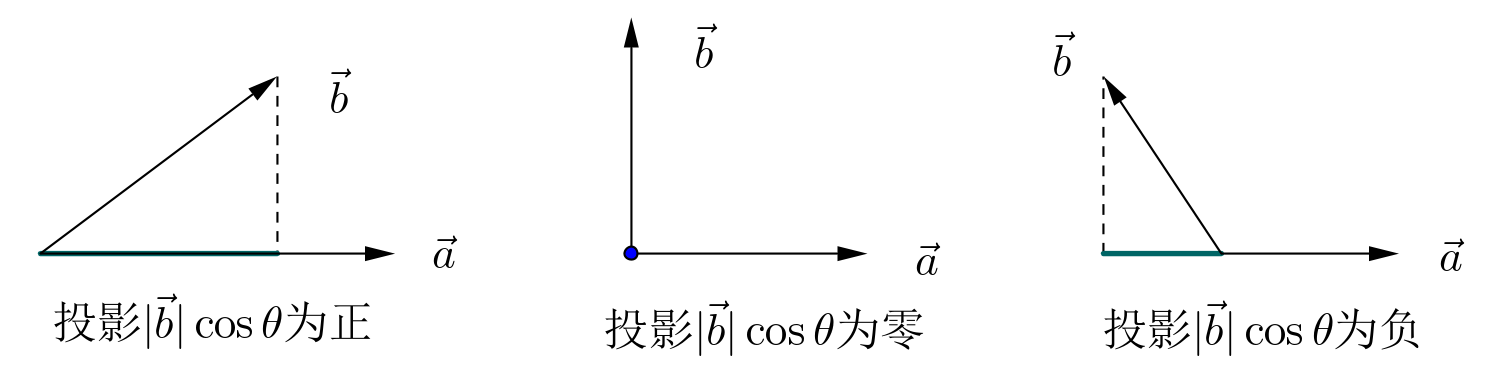
\includegraphics[width=4in]{d241-03.png}\pause

\begin{alertblock}{}向量 $\veca$ 与$\vecb$ 的数量积等于$\veca$ 的长度 $|\veca|$ 与$\vecb$ 在$\veca$ 的方向上的投影$|\vecb|\cos\theta$的积.\end{alertblock}
\end{frame}


\begin{frame}{数量积运算律}
  \begin{itemize}[<+->]
    \item $\veca\cdot\vecb=\veca\cdot\vecb$\quad 交换律
    \item $(\lambda\veca)\cdot\vecb=\lambda(\veca\cdot\vecb)=\veca\cdot(\lambda\vecb)$\quad 与数的结合律
    \item $(\veca+\vecb)\cdot\vecc=\veca\cdot\vecc+\vecb\cdot\vecc$ \quad 分配律
%等学习了坐标表示再证明
  \end{itemize}\pause
  \begin{alertblock}{注意}
    $(\veca\cdot\vecb)\cdot\vecc=\veca\cdot(\vecb\cdot\vecc)$ 成立吗?
  \end{alertblock}
\end{frame}


\begin{frame}
 \begin{exampleblock}{例3.求证:}\vspace*{-1em}
  \begin{align*}(1)&(\veca +\vecb)^2=\veca^2+2\veca\cdot\vecb+\vecb^2\\      
(2)&(\veca+\vecb)\cdot(\veca-\vecb)=\veca^2-\vecb^2
  \end{align*}
\end{exampleblock} 
\end{frame}


\begin{frame}\begin{exampleblock}{例4}
已知$|\veca|=6,|\vecb|=4$,$\veca$与$\vecb$的夹角为$60^\circ$,求$(\veca+2\vecb)\cdot(\veca-3\vecb)$.
\end{exampleblock}\pause
\begin{block}{解:}\pause
  $(\veca+2\vecb)\cdot(\veca-3\vecb)=\veca^2-3\veca\cdot\vecb+2\veca\cdot\vecb-6\vecb^2$\\\pause
$=\veca^2-\veca\cdot\vecb-6\vecb^2$\\\pause
$=|\veca|^2-|\veca||\vecb|\cos60^\circ-6|\vecb|^2$\\[.5ex]\pause
$=36-4\times6\times\dfrac12-6\times4^2$\\\pause
$=-72$
\end{block}\end{frame}


\begin{frame}\begin{exampleblock}{例5}
已知$|\veca|=3, |\vecb|=4$(且$\veca$与$\vecb$不共线),当且仅当$k$为何值时,向量$\veca+k\vecb$与$\veca-k\vecb$互相垂直?\end{exampleblock}
\begin{block}{解:}\pause
$(\veca+k\vecb)\cdot(\veca-k\vecb)=0\text{当且仅当}$\\\pause
$\veca^2-k^2\vecb^2=|\veca|^2-k^2|\vecb|^2=9-16k^2=0$, \\[1ex]\pause
$\text{所以,当且仅当}k=\pm\dfrac34\text{时}, $\\[1ex]\pause
$\text{向量}\veca+k\vecb\text{与}\veca-k\vecb\text{互相垂直}.$
\end{block}\end{frame}


\begin{frame}\begin{exampleblock}{例6}
  设$\veca,\vecb$是两个不共线的非零向量,且$|\veca|=|\vecb|=|\veca-\vecb|$,求向量$\veca$与$\veca+\vecb$的夹角
\end{exampleblock}
\begin{block}{解:}
$\cos\theta=\dfrac{\veca\cdot(\veca+\vecb)}{|\veca||\veca+\vecb|}\pause=\dfrac{\veca^2+\veca\cdot\vecb}{|\veca||\veca+\vecb|}$
\end{block}\end{frame}


\begin{frame}\begin{exampleblock}{例6}
  设$\veca,\vecb$是两个不共线的非零向量,且$|\veca|=|\vecb|=|\veca-\vecb|$,求向量$\veca$与$\veca+\vecb$的夹角
\end{exampleblock}\begin{block}{}
设$|\veca|=k$, \pause
则$|\vecb|=|\veca-\vecb|=k$,\\ \pause
因此$\veca\cdot\vecb=k^2\cos\dfrac{\pi}{3}=k^2/2$,\pause
$|\veca+\vecb|=\sqrt{(\veca-\vecb)^2+4\veca\cdot\vecb}=\sqrt3k$.\\[1ex]\pause
所以
$\cos\theta=\dfrac{\veca\cdot(\veca+\vecb)}{|\veca||\veca+\vecb|}=\dfrac{\veca^2+\veca\cdot\vecb}{|\veca||\veca+\vecb|}=\pause
\dfrac{k^2+k^2/2}{\sqrt3k^2}=\dfrac{\sqrt3}{2}.$\\[1ex]\pause
所以$\theta=\pi/6$.
\end{block}\end{frame}

%\begin{frame}\begin{exampleblock}{例7}
%设$x,y$轴正方向上的单位向量分别为$\veci$和$\vecj$,若$\veca+\vecb=2\veci-8\vecj$,$\veca-\vecb=-8\veci+16\vecj$,  求$\veca\cdot\vecb$.
%\end{exampleblock}\begin{block}{解:}
%\vspace*{-1cm}\begin{align*}\end{align*}\end{block}\end{frame}


%\begin{frame} \begin{exampleblock}{例8}
%设$\vecei$和$\veceii$是夹角为$45^\circ$的两个单位向量,且$\veca=\vecei+2\veceii$,$\vecb=2\veci+\veceii$试求$|\veca+\vecb|$的值.
%\end{exampleblock}\end{frame}

\begin{frame}{小结}
\setbeamercovered{transparent}
\begin{itemize}[<+->]\pause
  \item 向量的数量积的物理模型是力的做功.
  \item $\veca\cdot\vecb$的结果是个数量.
  \item 数量积满足交换律,分配律,与数的结合律,但是不满足结合律
  \item 利用数量积可以求两向量的夹角, 特别是可以判定垂直.
\end{itemize}
\end{frame}

\end{document}
过关课

反思第一:内容过多。准备了五个板块的内容,物理背景、定义、性质、运算律和应用,这使课堂内容远远超出了一节课的容量。


我有一个疑问,到底什么样的课堂是一节好课?把所有的知识都讲到位,就缺少给学生的思考空间;给学生太多的自主时间,学生又不知道自己干什么。这时候我应该以为恰到好处才好吗?但是任何人都知道偏向一方才好把握。那我选择让学生自己学习。来思考一下教师的使命。“师者,所以传道授业解惑也”,








